\section {Introduction}

    Depuis bientôt 4 ans, je suis mes études à l'Insa.
    La première chose que l'on m'a annoncé sur cette école, avant même son nom, était  l'importance de la composante humaine de la formation par rapport à d'autres établissements. Les PPH et l'importance de l'associatif en sont la preuve.

    Depuis bientôt 4 ans, j'ai eu l'occasion de travailler dans plusieurs associations : le Ski Club, l'AEDI, le BDE, les 24h,  pour ne citer que les plus importantes.
    Toutes ces expériences ont en commun ma passion pour les arts graphiques et la communication visuelle.

        
    
\section{But de la communication externe}

    Le but premier de la communication est de promouvoir les services, ou actions d'une association, d'une entreprise, d'un organisme.
    En résumé, de faire connaître une entité auprès du public.
    Dans le cas du ski club, il s'agira des sorties proposées et de la location. Pour les 24h, ce sera la festival, et les soirées préalables ; pour le BDE, les services et évènements organisés.
    Mais on peut prendre aussi l'exemple du forum Rhône Alpe, de la plupart des associations de département etc ...

    Tout le travail effectué en communication extérieure est principalement tourné vers la promotion des autres actions faites par l'association.
    Un seul contre-exemple me vient à l'esprit : les cartes de vœux envoyées par les 24h à ses partenaires.  Mais, en un sens, il est encore question de promotion, puisque cela contribue à garder de bonnes relations ainsi qu'à pérenniser les partenariats commerciaux.


\section{Mes expériences dans l'associatif}

    \subsection{Le ski club}
        
        Depuis que je suis enfant,  j'ai la chance de skier chaque hiver. Pour poursuivre cette activité durant mes études, je me suis inscrit dès ma première année comme membre actif du Ski club.
        
        L'ancien webmaster quittait l'Insa l'année de mon arrivée, je me suis donc proposé de reprendre le site de l'association pour le maintenir.
        Ce fut ma première expérience relative à la communication dans l'associatif.
        J'ai entièrement reconstruit le site web, pour améliorer la visibilité en ligne de l'association.
        
        Le site comportait des informations concernant l'organisation des sorties, du weekend à venir, ainsi que sur la location ou l'entretien de matériel.
        
        Je ne fais plus partie du ski-club, le site a été récemment replacé par une plate-forme web plus pratique à maintenir. 
        
    \subsection{L'AEDI}
        
        Il serait faux de dire que je suis membre de l'AEDI. Je n'ai fait que proposer mon aide en cas de besoin.
        Mais j'ai eu l'occasion de dessiner un visuel de T-Shirt distribué aux \emph{bizuth} lors du weekend d'intégration, et différentes affiches pour le barbecue de fin d'année.
        
        Ces travaux étaient d'une durée très courte, et il y avait peu de travail collaboratif, j'en parlerai donc peu par la suite.
        
    \subsection{Les 24 heures de l'Insa}
        
        Cela fait 2 ans que je suis dans l'équipe communication des 24h de l'INSA, et c'est probablement pour cette association que j'ai fourni le plus de travail.
        Durant ces deux années,  j'ai dessiné un certain nombre de ressources qui ont été réutilisées sur différents supports, tels que les programmes, les gobelets, les T-Shirts, les affiches etc ...
        J'ai également participé, entre autres, à l'élaboration des affiches journées et concerts.
        
        J'en tire de bonnes expériences notamment en ce qui concerne la suivi d'un projet sur une plus longue durée.
        Le fait de travailler par équipe nous amène souvent à présenter nos idées et notre travail, à prendre des décisions communes et à remettre en question des idées, ou des ébauches.
        
    \subsection{Le BDE}
    
        J'ai également collaboré à plusieurs projets avec l'équipe communication du BDE.
        Cependant, ayant intégré l'équipe en cours d'année, je n'ai pas eu l'occasion de faire des travaux très significatifs.

\section{Observations}

    La première observation que j'ai pu faire aussi bien au sein de l'équipe com du BdE que des 24h, est que la communication externe n'est pas toujours à la hauteur pour promouvoir les efforts fournis par les autres services ; soit à cause d'un retard, d'un manque de moyens, ou d'un manque d'efficacité.

    \subsection{BdE}

        Par exemple, au BdE, en comparaison à la médiatisation que l'on peut voir dans la plupart des entreprises, le service de communication est en sous-effectif. Il devrait être plus important afin d'être plus productif, plus efficace et mieux faire connaitre les services proposés aux étudiants.

        Cependant, je suis conscient que ce n'est pas comparable à une entreprise commerciale, dont la survie dépend en grande partie de sa visibilité.
        Les services du BdE ne pâtissent pas d'une mauvaise visibilité, et rencontrent toujours le public étudiant attendu.
    
    \subsection{24 heures de l'Insa}
        
        En revanche, la communication aux 24h est plus importante et mieux planifiée, parce qu'indispensable à la manifestation, mais elle n'est souvent pas assez organisée pour avoir des ressources graphiques vraiment utilisables d'une année sur l'autre.
        
        Le planning des tâches est organisé de telle manière que celles qui demandent le plus de travail (T-Shirt et Affiches) sont réalisées en dernier.
        Tandis que des réalisations plus simples, telles que les campagnes de pré-communication, ou des affiches de soirées moins importantes (soirées de séléction des groupes, soirée SIDAction etc ...) sont plannifié avant.
        Il en résulte que le travail de cohérence graphique n'apparaît important que tard dans le planning, ainsi, l'idée de réutiliser des ressources n'est pas immédiate.

        Bien qu'un effort soit fait de ce côté-là. Pour donner un exemple, les photos prises sur la manifestation sont souvent réutilisées d'une année sur l'autre dans plusieurs supports de communication, notamment le site web, ou les plaquettes destinées aux sponsors.
        
        Cette remarque peut être nuancé en notant que les 24h bénéficient déjà d'une grande notoriété auprès d'un certain public, et une campagne de communication faite en urgence, et pas aussi travaillée qu'attendue ne nuira ni au festival, ni à son image. Le but est plus d'informer le public que d'attirer de nouvelles personnes.
    
\section{Déboires : les pièges à éviter}

    Je vais revenir sur plusieurs gros projets, en analysant quelles étaient les difficultés, les enjeux, et pourquoi ces projets n'ont pas abouti ou ont connu des difficultés.
    
    \subsection{La bâche de la MdE}
    
        Le BdE ayant un partenariat important/conséquent avec Perstil, ceux-ci nous proposèrent une impression gratuite sur une bâche de 8m par 1m, avec pour seule contrainte, un bandeau publicitaire au bas de l'affiche. 
        La décision fut prise de placer cette bâche au devant de la MdE, sur la rambarde du balcon, pour attirer un peu plus l'œil et signaler la présence de la MdE.
        Quand je suis arrivé dans l'équipe, cette proposition était déjà lancée depuis quelques année, mais personne ne s'était mis à la tâche.
        Je me suis donc proposé pour travailler dessus pendant l'été. Et après quelques réunions, le thème choisi serait "Urbano-floral".
        
        J'ai très vite réalisé, face à une tâche et un travail aussi importants, que le thème ne pouvait se résumer à deux mots.
        
        Ainsi, je commencé à travailler avec des idées en tête. Les membres de l'équipe étaient en désaccord avec la plupart des ébauches que je présentais, chacun ayant une vision différente du thème. Le projet finit par stagner, un consensus ne pouvant se dégager.
        
        Il aurait été souhaitable de mieux définir un style visuel ainsi que  le résultat attendu, par exemple en se posant les questions suivantes :
        Pourquoi faire ce travail ? Qu'est qui est attendu du résultat ? Dans quel registre peut-on se placer, et à quoi ressemblera sommairement le résultat final ?
        
    \subsection{Les affiches Journées et Concerts des 24h}
        
        Un des travaux les plus importants pour l'équipe communication des 24h est la réalisation des affiches Journées et Concerts.
        Ce sont deux affiches imprimées au format B1, en grand nombre et qui sont en grande partie responsables de la visibilité des 24h sur Villeurbanne, Lyon et ses alentours.
        
        Chaque année, des propositions de thèmes et des ébauches d'affiches sont présentées plusieurs mois avant la manifestation, afin que l'équipe entière des 24h puisse juger et voter pour un thème.
        L'an dernier, les deux idées qui s'étaient démarquées étaient une reprise des lapins suicidaires de Andy Riley, et un thème dont la ligne directrice était l'aspect BD.
        Nous avons alors choisi d'utiliser les 2 thèmes.

        J'avais une idée très précise de ce que je pensais faire, et elle semblait plaire à l'équipe.
        
        Entre-temps, l'idée des lapins suicidaires a été abandonnée, pour des raison évidentes.
        Nous avons donc remplacé dans la précipitation les lapins par des pandas, image plus positive. (Ce n'est que trop tard que nous avons réalisé le lien évident avec l'association \emph{la semaine asiatique}.)
        
        J'ai commencé à proposer des ébauches, et le travail avançait bien.
        Au fur et à mesure que j'avançais, des remarques m'ont été faites dans le but d'améliorer certains détails.
        Mais plus le travail avançait, plus le nombre de remarques augmentait, et plus j'approchais du résultat final, plus il semblait déplaire.
        C'est comme ça que, quelques jours avant l'envoi à l'imprimeur, il a été décidé de recommencer à zéro pour produire une affiche différente.
        
        Je ne pense pas que cette deuxième affiche faite dans la précipitation soit mieux réalisé que celle effectué au préalable.
        En revanche, présenter à l'équipe un travail fini, et non des ébauches, a été décisif pour qu'il soit  accepté plus facilement.
        Chacun ne s'est pas projeté dans l'ébauche pour imaginer un travail fini et être ensuite  déçu.
        Au contraire, un travail fini et intègre est difficilement critiquable, puisque il est plus compliqué de cerner précisément les éléments à modifier pour l'améliorer.
        
        Je pense donc que bien qu'il faille bien faire la distinction entre des remarques concernant des améliorations possible ( meilleure visibilité, meilleure cohérence, meilleur équilibre ... ) et des remarques personnelles de goût.
        Il faut faire preuve d'une sorte de bon goût universel, et ne pas s'arrêter à des préférences personnelles.
        
        Il existe des règles d'utilisation de typographies et de couleurs, qui sont prouvées  et approuvées. Elles peuvent découler du bon sens, et de l'expérience mais les suivre peut faire gagner du temps et une certaine expérience.

        
        Pour mieux cerner nos problèmes et améliorer notre démarche, je me suis penché sur la façon de procéder du festival Rock'n'Solex, qui est très proche des 24h de l'Insa (festival étudiant organisé par l'Insa de Renne).
        Ils ne travaillent pas eux-même sur l'affiche, mais lancent un concours. Ils ont une réputation suffisante pour que les concurrents produisent des travaux de bonne qualité.
        Quelques modifications mineures sont faites sur l'affiche gagnante, puis c'est l'impression.
        
        La grande différence, c'est qu'ils choisissent parmi des travaux déjà aboutis, complets, qui ont déjà un certain caractère et une intégrité. 
        
        Je peux en conclure qu'au delà de l'affiche, c'est véritablement une charte graphique qu'il faut définir, sur laquelle travailleront les graphistes concurrents pour la présenter sous forme d'affiche. Ensuite, il est aisé de reprendre des éléments clés pour d'autres supports tels que les flyers, les programmes ou les gobelets.
        
        Je ne pense pas qu'un concours d'affiches récolte les résultats escomptés, et il est impossible de demander à plusieurs personnes de travailler chacun sur une affiche différente pour ensuite choisir la meilleure.

        Cependant, tout en gardant la présélection du thème par l'équipe complète, il serait préférable de commencer très tôt à réfléchir sur l'affiche avec un groupe de personne restreint (2 ou 3), jusqu'à sa finalisation. Ainsi le thème est illustré par une ambiance graphique, source d'inspiration pour les travaux futurs.
        

\section{Relations \& Expériences humaines}

    L'associatif apporte énormément en terme de relations humaines. Que ce soit vis à vis des autres étudiants qui travaillent conjointement, ou vis à vis des prestataire de service embauché, des sponsors etc ...
    
    Pour ma part, je n'ai pas eu beaucoup l'occasion d'être en relation avec les intervenant extérieur.
    Mais j'ai eu beaucoup plus d'occasion de collaborer avec les autres étudiants.
    
    La collaboration au sein de l'équipe est assurée par 2 choses, les réunions d'équipe, et les communications par mail.

    \subsection{Les réunions}

        Tous les mois, toutes les 2 semaines, ou toutes les semaines, la fréquence des réunion varie en fonction de la charge de travail, et l'équipe.

        Au 24h, la réunion était fixé toutes les semaines entre midi et 2 heures, tandis qu'au BdE, l'agenda étant plus souple, les réunion n'était pas fixes mais s'organisaient a l'avance, souvent entre midi et 2 heures, toutes les 2 ou 3 semaines.

        Lors d'une réunion, le principal objectif est de faire le point rapidement sur les projets existant, et de présenter les nouveaux projets. Les réunions sont tenus par le responsable d'équipe dont le rôle est simplement de coordonner l'équipe, en s'assurant que tout ce qui doit être fait, l'est dans les temps.
        
        Le responsable d'équipe rappel brièvement les échéances a tenir pour chaque projet, rappel les projets les plus en retard, pour lequel il faut le plus de travail etc ...
        
        Il n'est pas rare, lorsqu'un projet est en retard, que l'équipe réfléchisse dessus pendant la réunion pour sortir un brouillon qui sera réalisé plus tard.
    
    \subsection{Les échanges de mails}

        Les réunions hebdomadaires en elles-même ne sont pas suffisante. Une grande partie du travail collaboratif se repose sur l'échange de mails.
        Il est plus difficile de montrer son travail (souvent numérique) pendant la réunion qu'en l'envoyant par mail a l'équipe afin d'avoir l'avis collectif.

        C'est par mail que la plupart des décisions sont prises.
        
\section{Conclusion}

    De manière générale, dans l'associatif le travail fourni est important. Je pourrais estimer à 10\% le ratio de travaux qui seront effectivement publiés.

    Il y a effectivement une part du travail qui est dédiée à des essais, ou soumis à des sélections, une part importante du travail qui ne sera jamais aboutie et abandonnée en cours de route. Pour une meilleure efficacité, le but est donc de réduire au maximum cette part.

    La principale cause de ce gaspillage est la méthode employée : en effet, il est plus facile de travailler sur une production, de la finir, puis d'en commencer une autre, et ainsi de suite. Ce travail est parallélisé entre plusieurs personnes, pour être plus rapide.

    \subsection{L'intérêt d'une charte graphique}
    
        S'obliger à établir une charte graphique claire et fournie, permettrait de réduire grandement ce gaspillage.
        Il serait plus judicieux, à mon sens, de travailler sur un ensemble de ressources graphiques réutilisables plutôt que de travailler production par production.
        Ainsi, pour chaque production, il ne reste plus qu'à déterminer la mise en page et  apporter quelques adaptations.

    \subsection{Mise en pratique}

        Dans le cas du BdE, cette charte graphique est présente, car la communication s'étale tout au long de l'année, et il est indispensable d'avoir une cohérence visuelle.
        La campagne la plus récente, pour la Coop, est une série d'affiches sur le même modèle avec un texte et une illustration différente.
        
        En revanche, dans le cas des 24h,  le thème changeant chaque année, la production graphique est entièrement à refaire.
        C'est la raison pour laquelle, pendant les 2 ans où j'ai participé à cette équipe, le travail de chacun s'éparpillait dans un nombre incroyable de travaux très intéressants, mais peu, voire pas cohérents une fois rassemblés, donc inutilisables.
        
        Le fait que les travaux les plus importants soit effectués en dernier, pousse l'équipe à effectuer les premier travaux rapidement, sans penser à produire des éléments réutilisables.
        D'une année sur l'autre, le thème change, il n'est donc pas possible de réutiliser la plupart des ressources graphiques ; en revanche, il serait bénéfique de travailler sur un ensemble de ressources réutilisables tout au long d'une année.

\newpage

\section{Portefolio}

    Je présente ici différents travaux qui illustrent le mieux mon travail, et les évolutions que suit un projet.
    \subsection{BdE}
        \begin{center}
            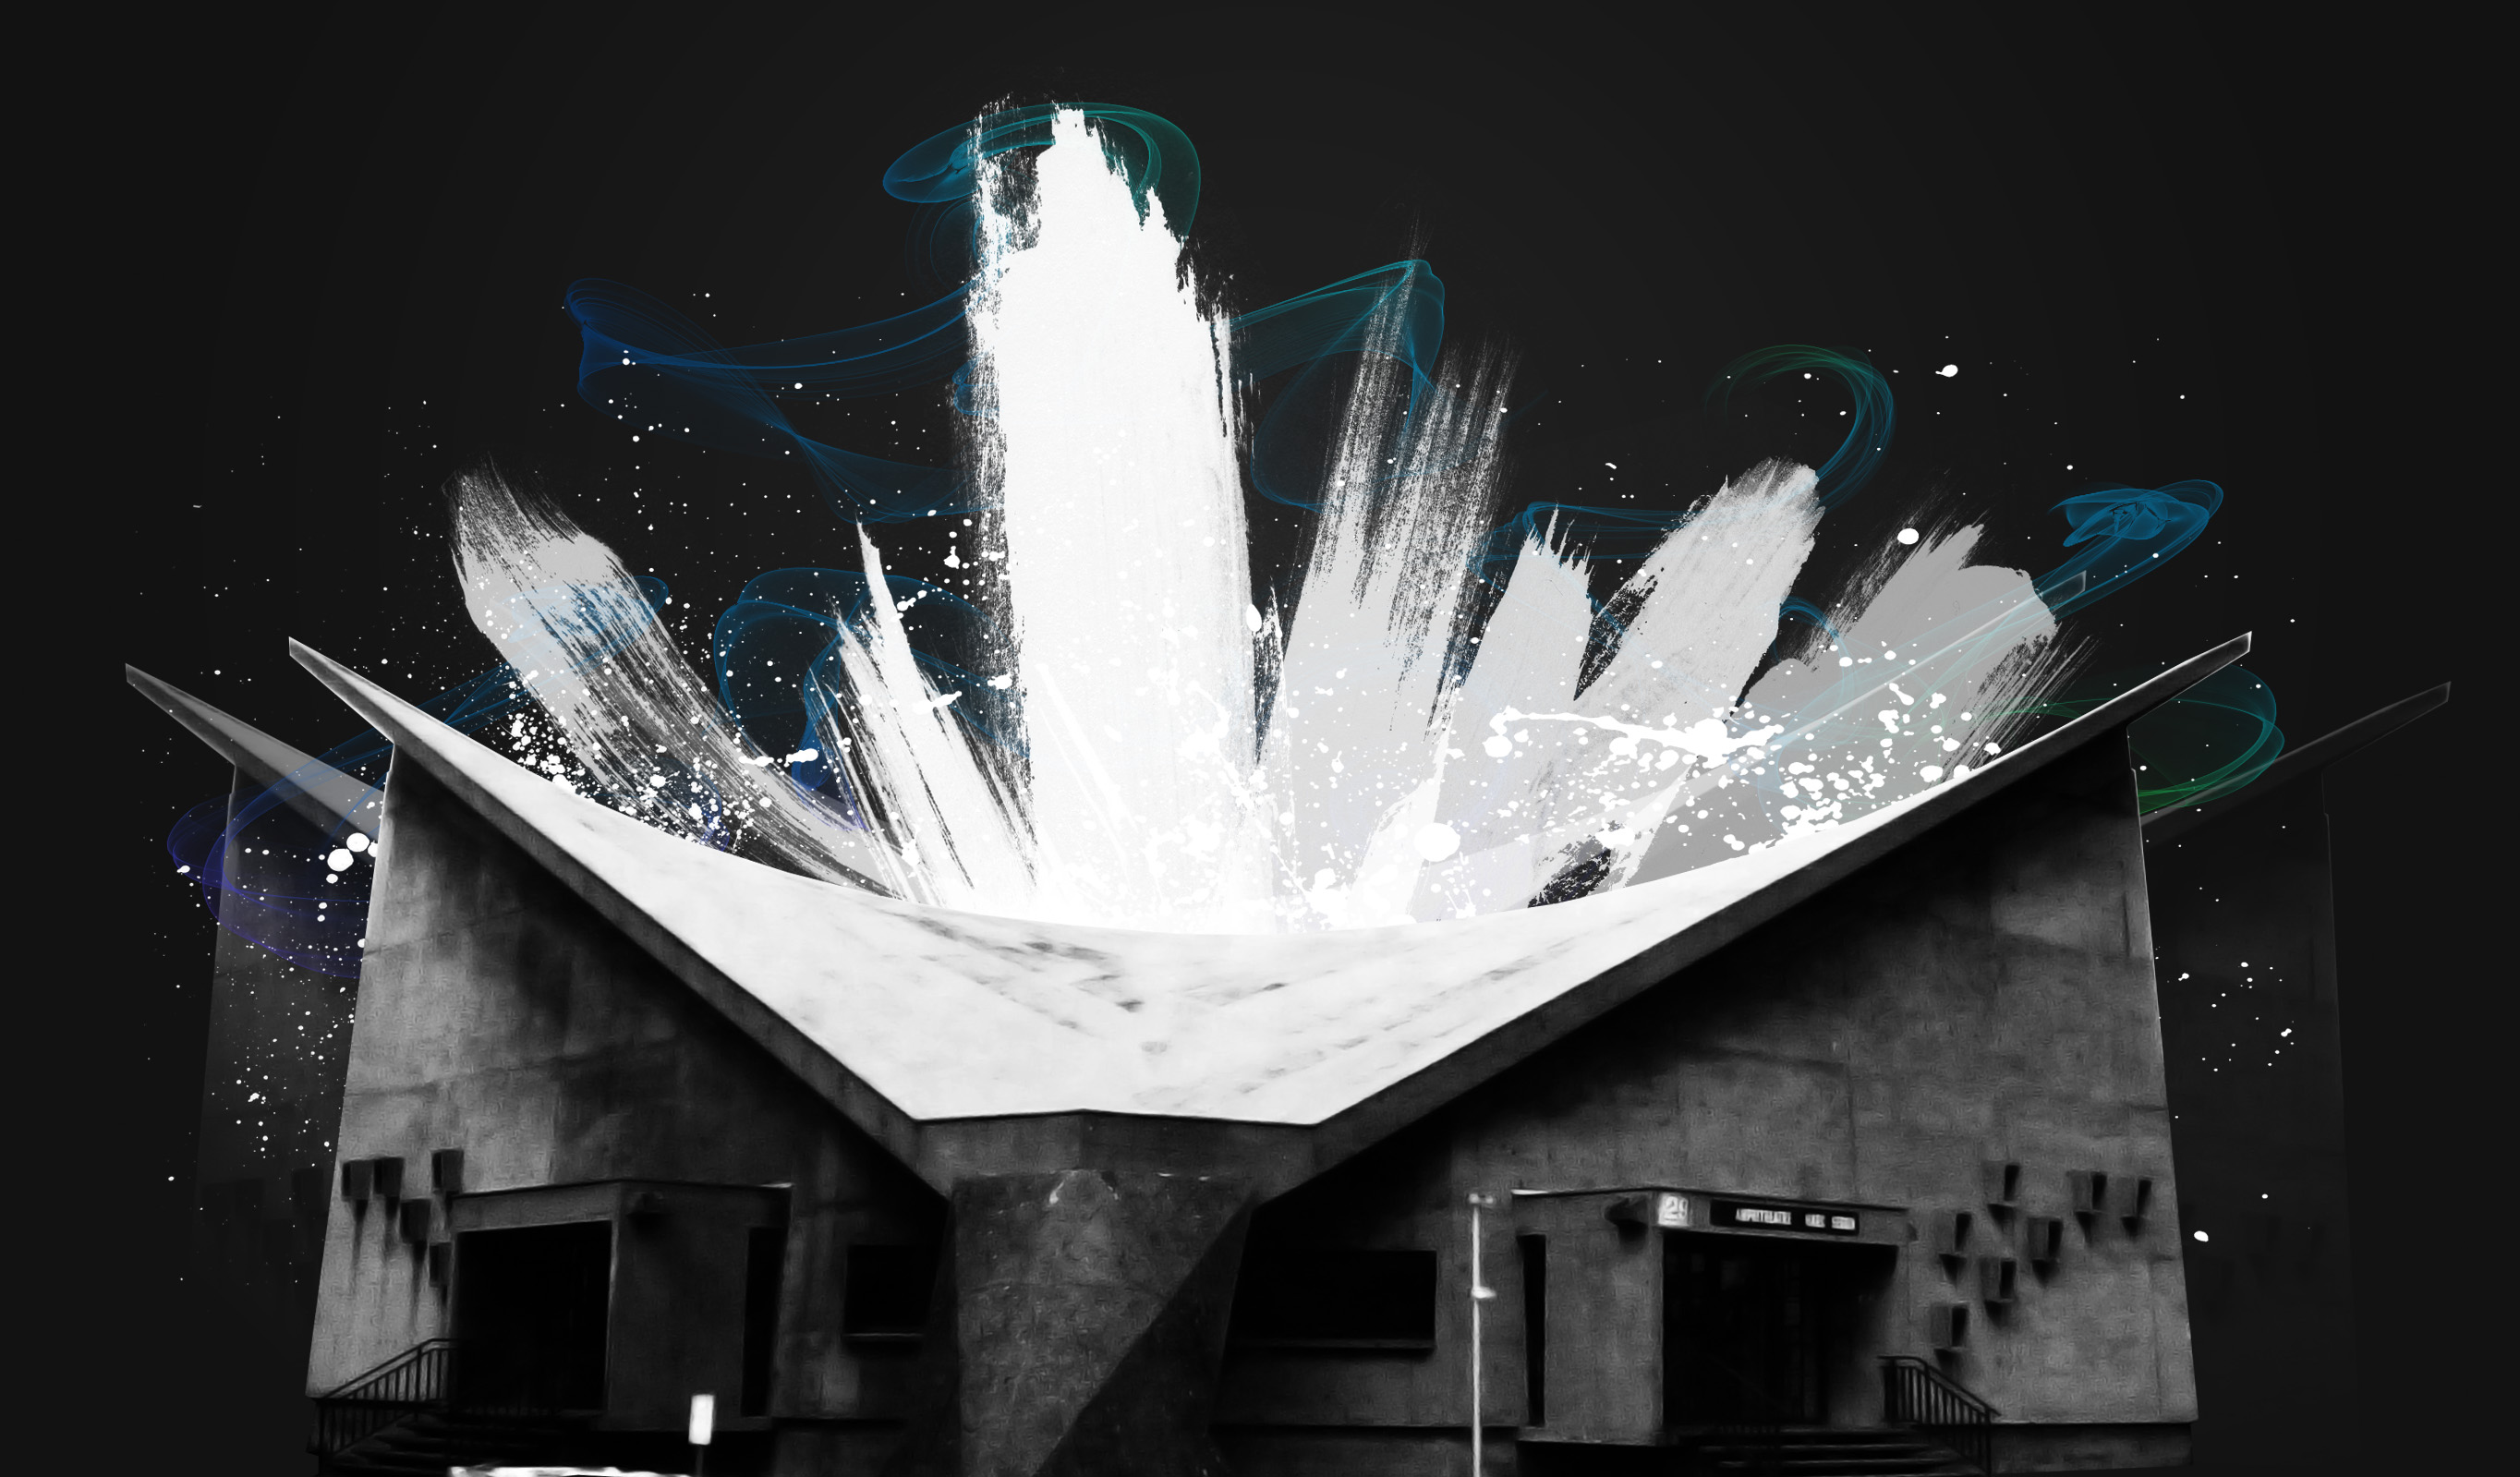
\includegraphics[width=\textwidth]{img/amphi.jpg}\\
        \end{center}
        
                    Un des fil conducteur de ce travail, était de reprendre des éléments du campus avec un certain style graphique afin de donner une image représentative du campus au travers de la bannière.
	        C'est pourquoi j'ai essayé ici de reprendre un des amphi du campus, et en lui appliquant quelques formes vectoriels, et quelques motifs, essayer d'obtenir l'équilibre urbano-floral attendu.
            C'est une des esquisse les plus réussi, mais loin d'être la plus aboutie, malheureusement.

        \begin{center}
            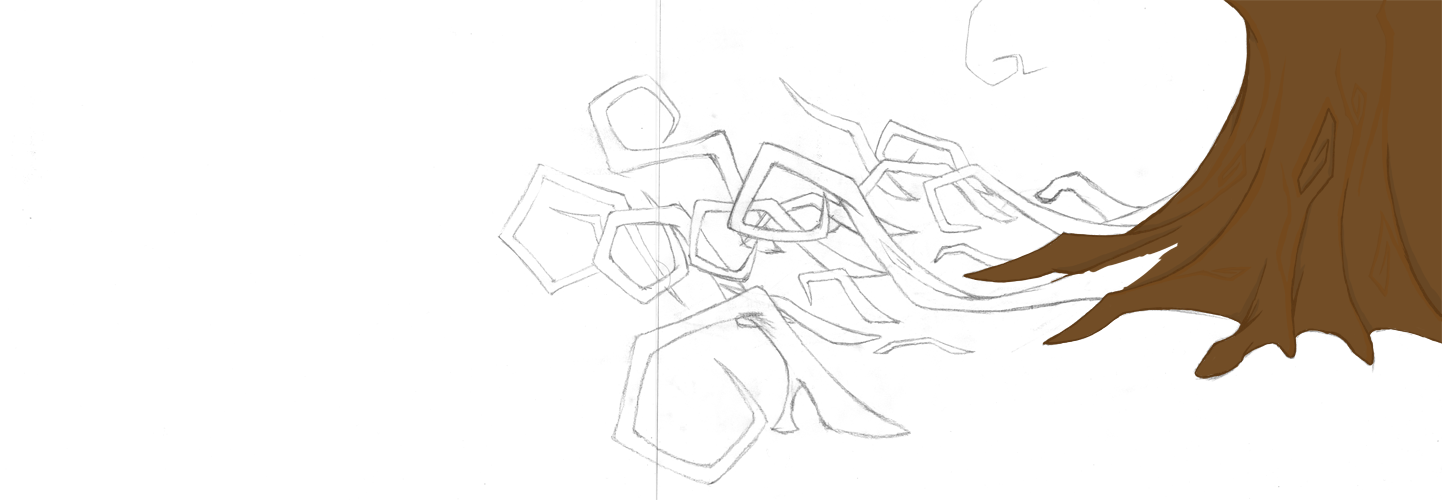
\includegraphics[width=\textwidth]{img/arbre.png}
            
\includegraphics[width=\textwidth]{img/mde.png}
            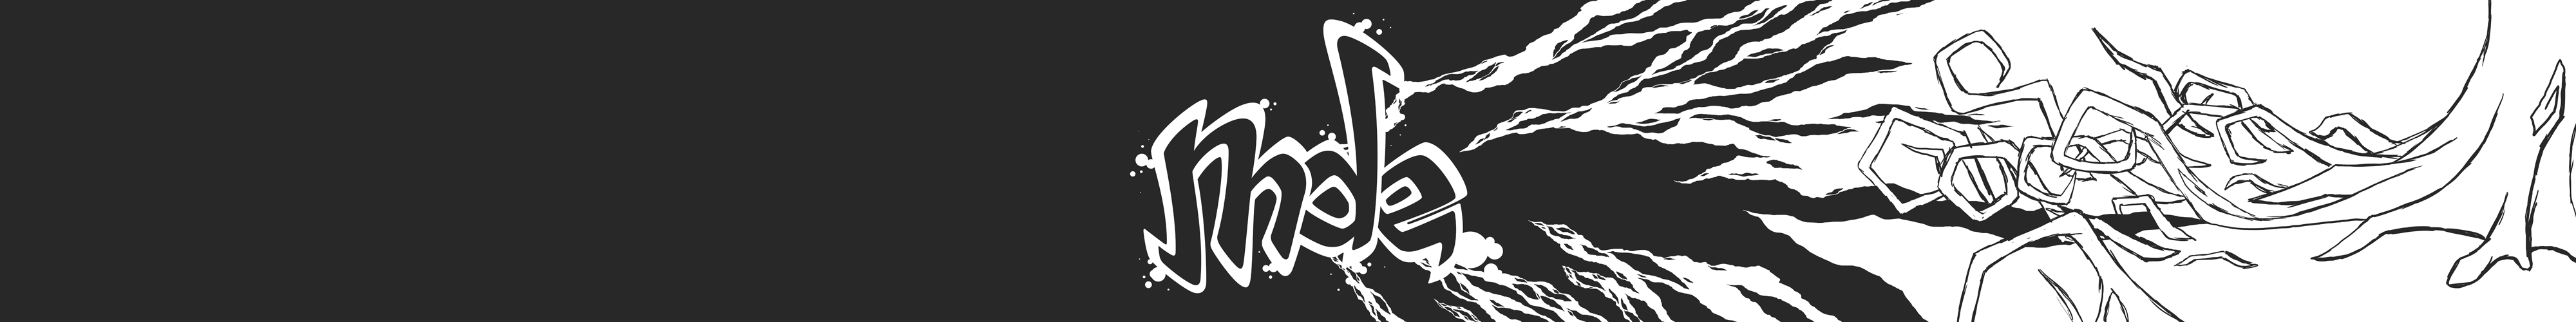
\includegraphics[width=\textwidth]{img/mde+arbre.png}
        \end{center}
        
                    Après avoir eu une bonne impression avec l'esquisse de l'amphi, j'ai essayé de créer une trame qui pourrait se prolonger sur toute la frise, afin d'installer une certaine cohérence.
Je pensais ensuite y incorporer divers éléments similaire à l'esquisse de l'amphi.
            L'arbre aurait des racines qui aboutirait en formes plus urbaine pour s'entremêler avec des graffitis ou d'autres motifs dans une vrai continuité.
            
    \subsection{24h de l'Insa}
    
        \subsubsection{36ème édition - 2010}
    
            \begin{center}
                \fbox{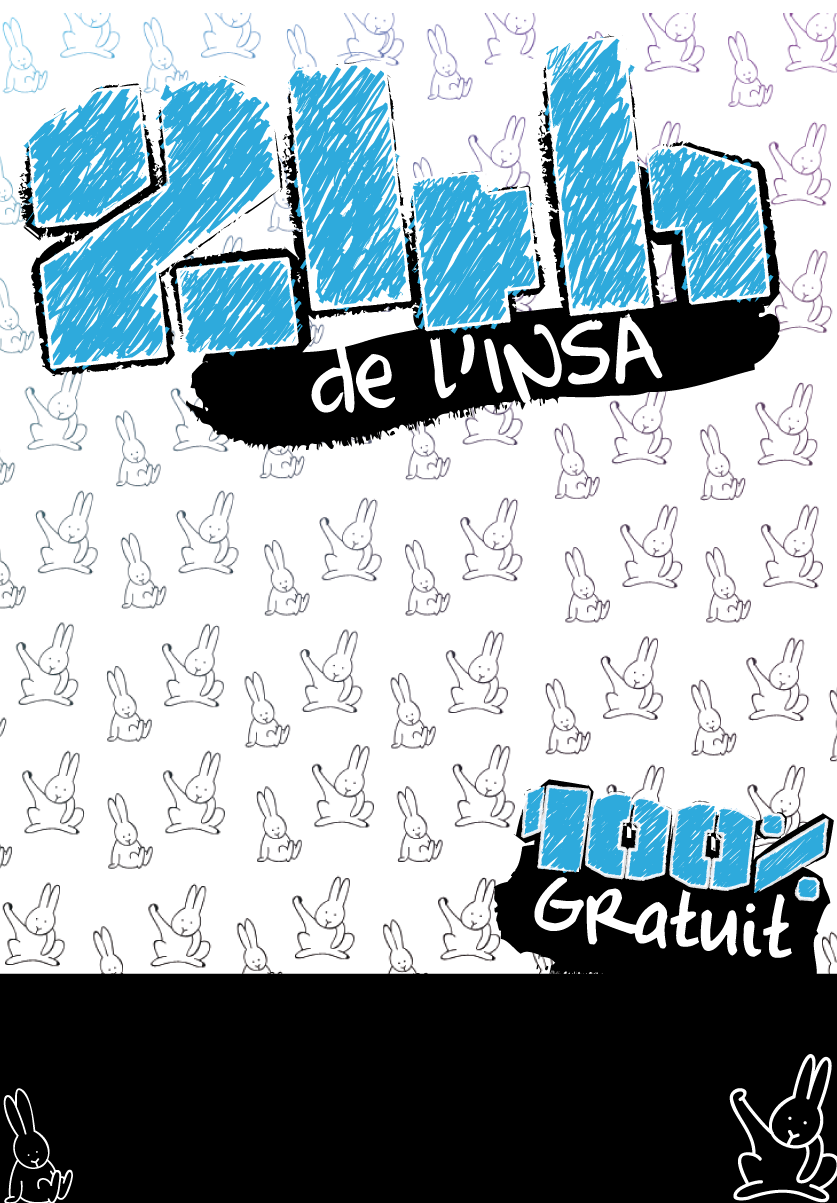
\includegraphics[width=0.3\textwidth]{img/preAffiche.png}}
                \fbox{
\includegraphics[width=0.3\textwidth]{img/preAffiche_panda.png}}
                \fbox{
\includegraphics[width=0.3\textwidth]{img/preAffiche_panda_2.png}}\\    
                \fbox{
\includegraphics[width=0.3\textwidth]{img/preAffiche_panda_2leaf_date1.png}}
                \fbox{
\includegraphics[width=0.3\textwidth]{img/preAffiche_panda_2leaf_date2.png}}
                \fbox{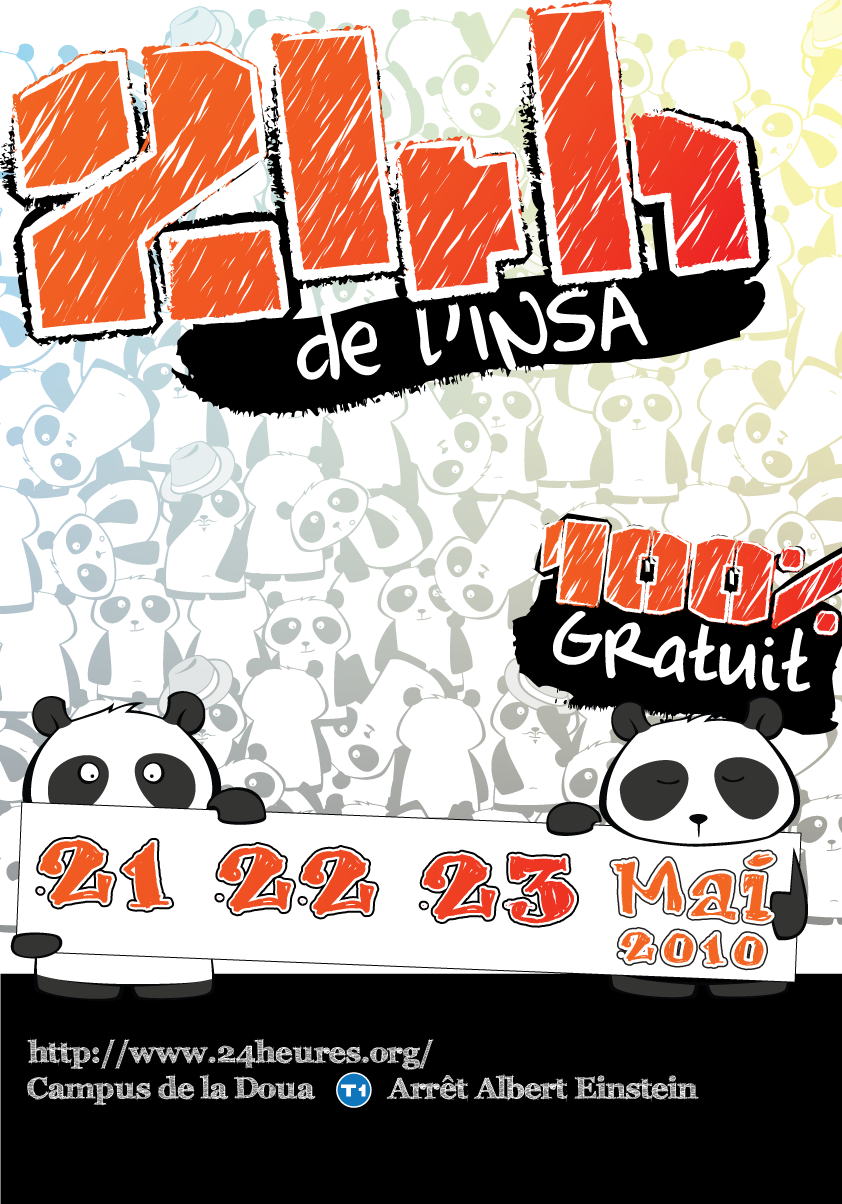
\includegraphics[width=0.3\textwidth]{img/preAffiche_panda_2hot.png}}\\
                \fbox{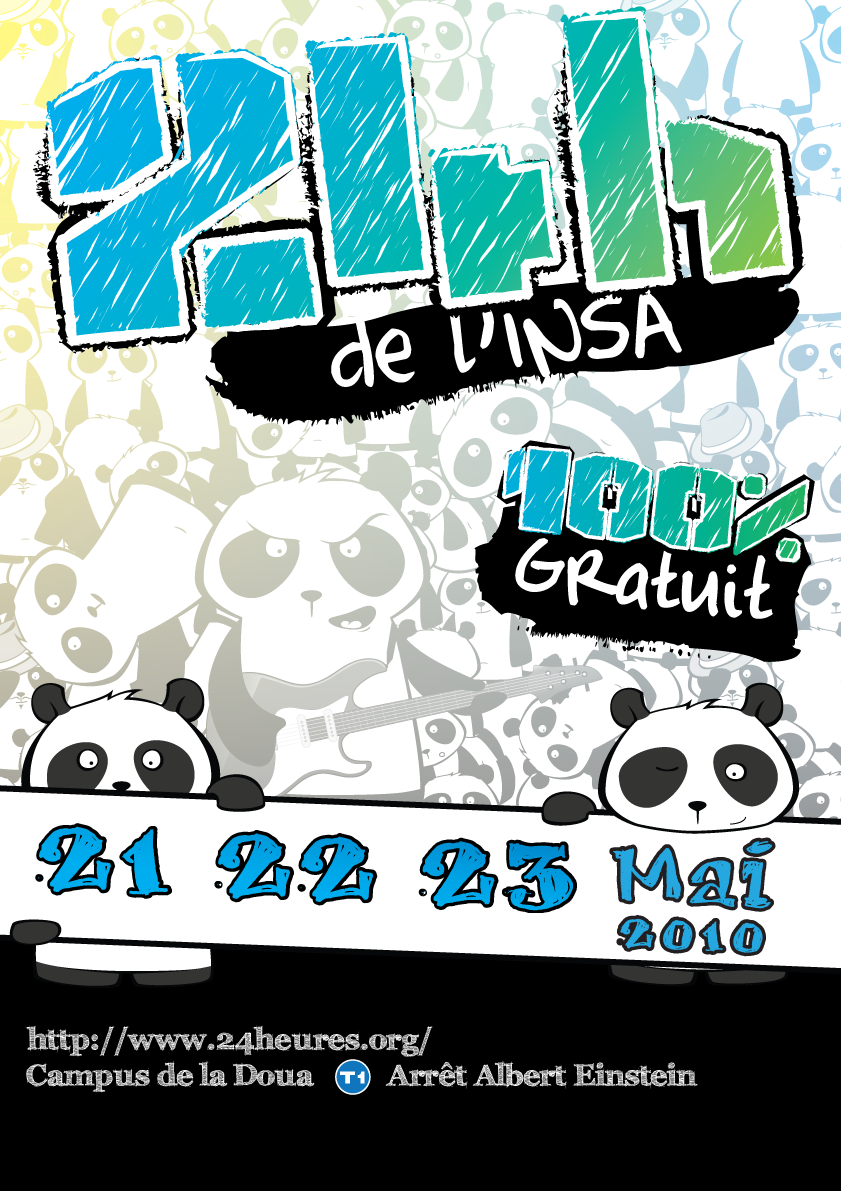
\includegraphics[width=0.3\textwidth]{img/preAffiche_panda_3.png}}
                \fbox{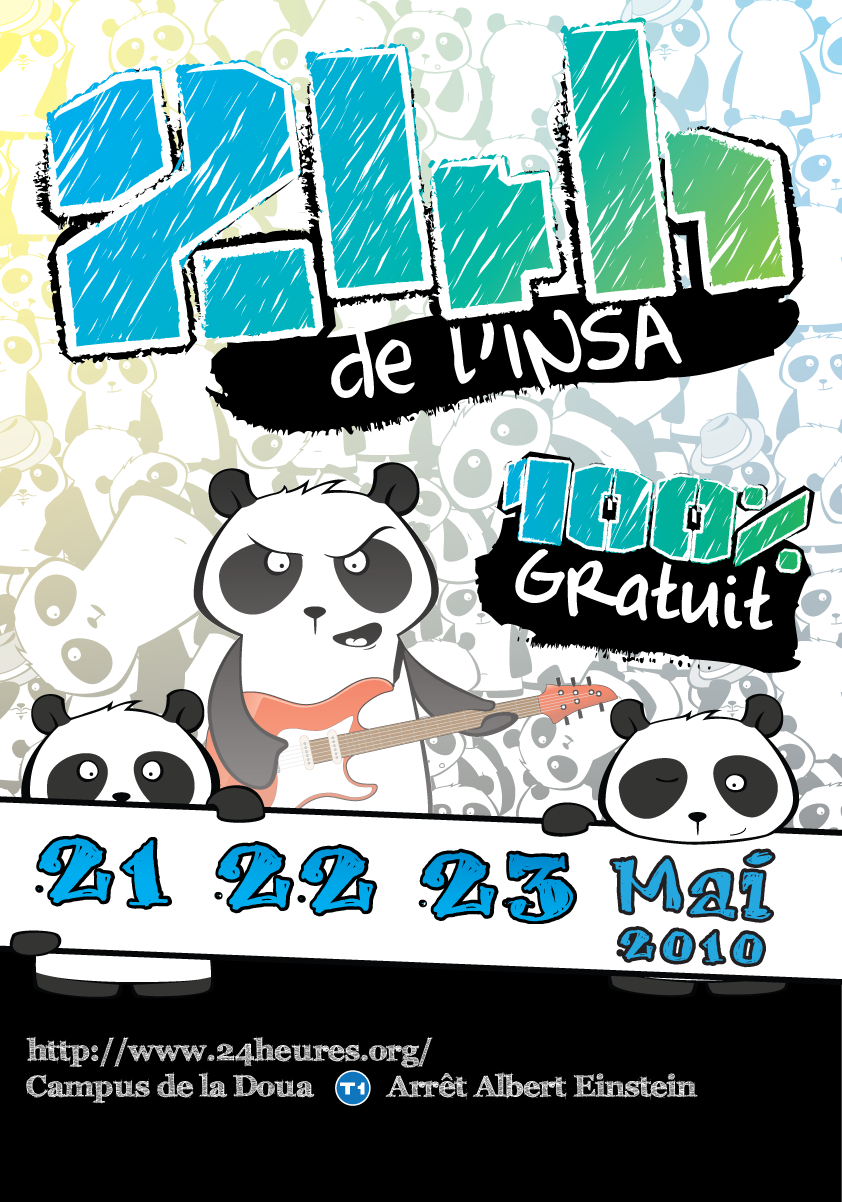
\includegraphics[width=0.3\textwidth]{img/preAffiche_panda_3-2.png}}
                \fbox{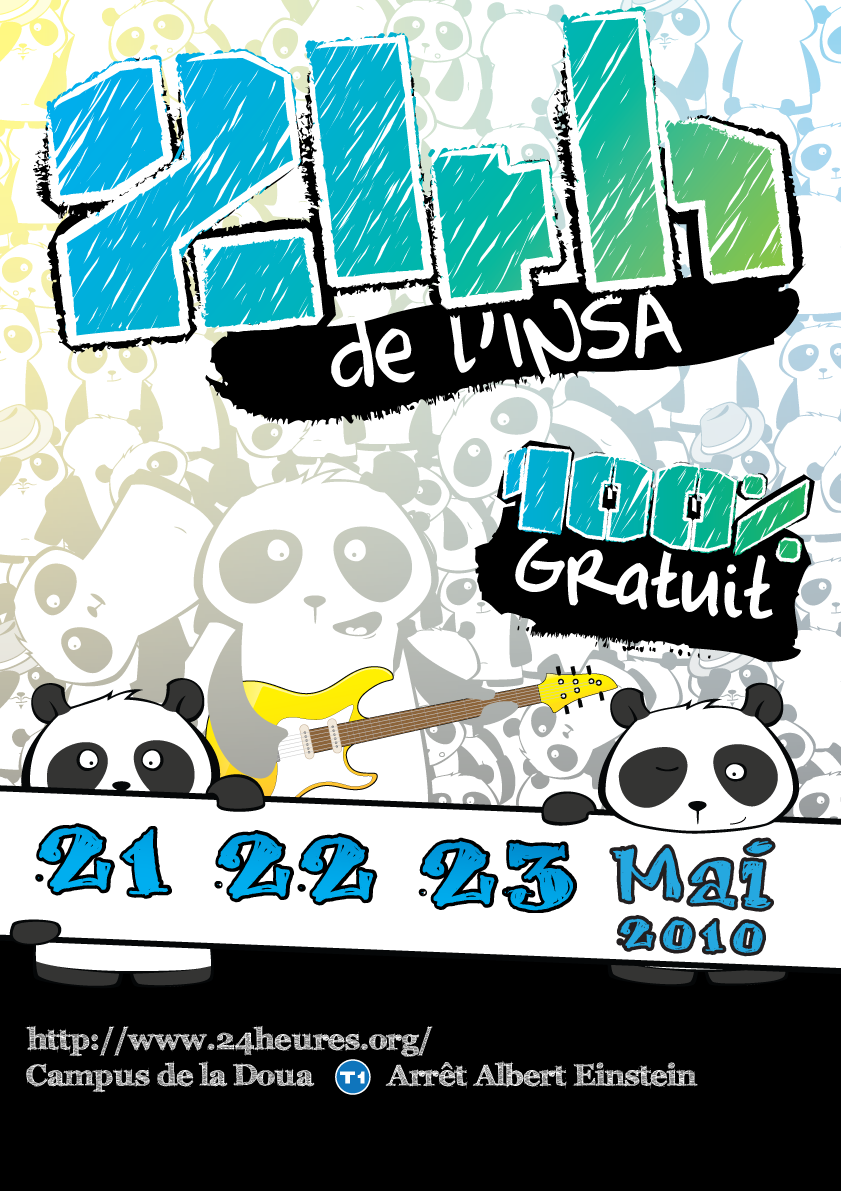
\includegraphics[width=0.3\textwidth]{img/preAffiche_panda_3-3.png}}\\
            \end{center}
            
                            Ayant participé du début à la fin à la production de l'affiche de la 36ème édition des 24h, j'ai pu suivre la progression du travail.
                Il est intéressant de noter les modification apporté tout au cours de l'année.
                
                On voit que la première ébauches comportait encore les lapins suicidaire de Andy Riley, abandonné par la suite. Puis la progression, avec différentes modifications à chaque fois.
                On peu noter, par exemple, le choi des couleurs qui à légerement changé.
                Différents tests sur la date pour améliorer sa visibilté et sa lisibilité, en modifiant le contour, les couleurs etc ...
                Le second panda qui tiens la pancarte de la date se réveille au milieu de la production pour donner une image plus dynamique au festival.
                Les dernières modifications portaient sur la visibilité du personnage principal de l'arrière plan.
                Le but étant de rendre l'affiche la plus vivante et dynamique possible par l'ajout d'une scène/ d'une action, tout en gardant le reste des informations lisibles et captivante.
            
            \begin{center}
                \fbox{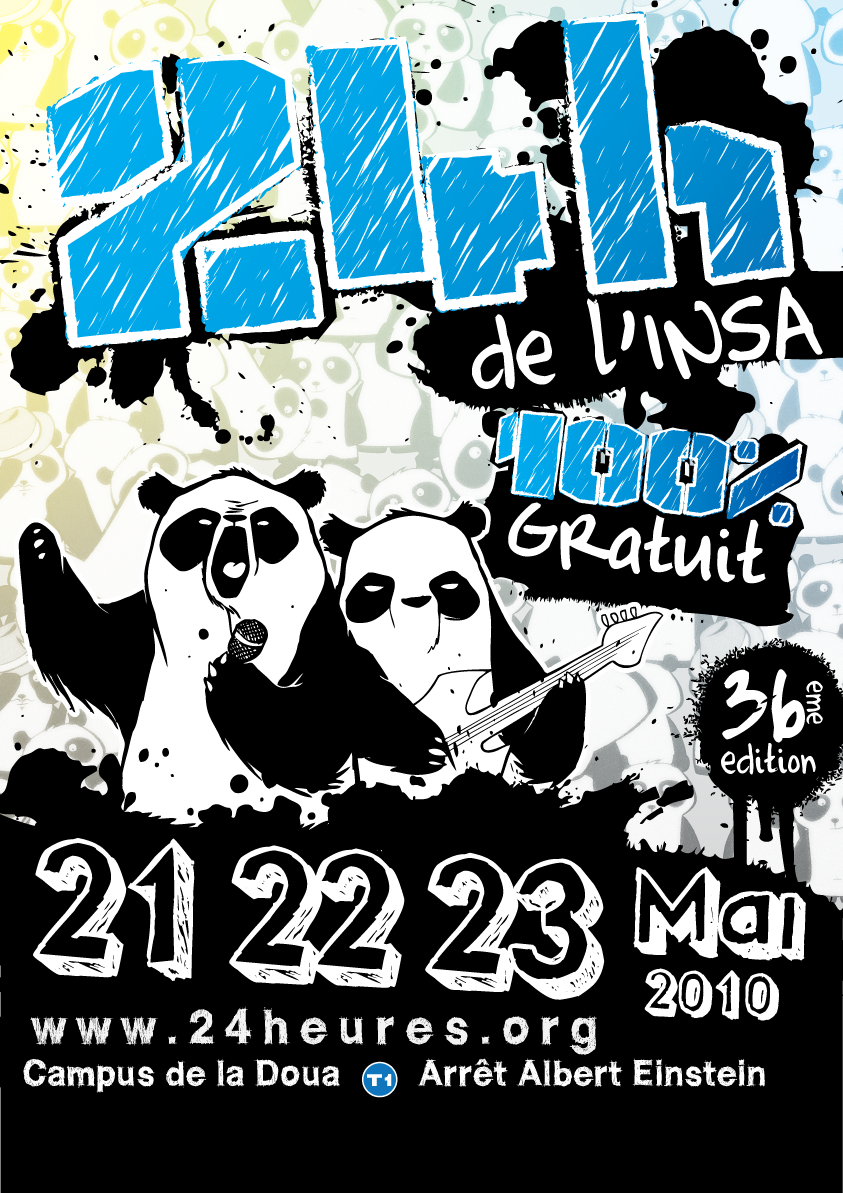
\includegraphics[width=0.48\textwidth]{img/affiche_concert.png}}
                \fbox{
\includegraphics[width=0.48\textwidth]{img/affiche-concerts-v4-flat2.jpg}}\\
            \end{center}
            
                            Sur les quelques derniers jours avant l'impression, les modifications allaient très vites, et je n'ai pas gardé toutes les esquisses présenté, mais à la fin j'ai présenté mon travail, que j'ai recentré sur les 2 pandas, et sur une ambiance plus \emph{trash}, contrastant avec les couleurs très fluos, et les pandas de l'arrière plan beaucoup plus innocent.
                En parallèle, une autre version à été réalisé, et finalement retenu.
                Bien qu'on retrouve certains éléments à l'identique, l'ambiance généré n'est pas du tout la même.
                Les couleurs vive, et le fond bleu sont plus chaleureux et accueillant que le fond très clair de l'affiche précédente.
                Cependant, les couleurs ne s'accordent pas très bien entre elle. On ne retrouve le violet ou le vert des spots nulle part. L'utilisation de la police Comic Sans Ms pour le site web, en revanche, est beaucoup plus critiquable.
                Afin de rendre les pandas centraux moins agressif, et plus sympathique, des pupilles ont été rajouté à leurs yeux.
                Il est interessant de noter comme un détails aussi infime que ça, peut complètement changer l'ambiance dégagé.
            
        \subsubsection{37èeme édition - 2011}            
            
            \begin{center}        
                \fbox{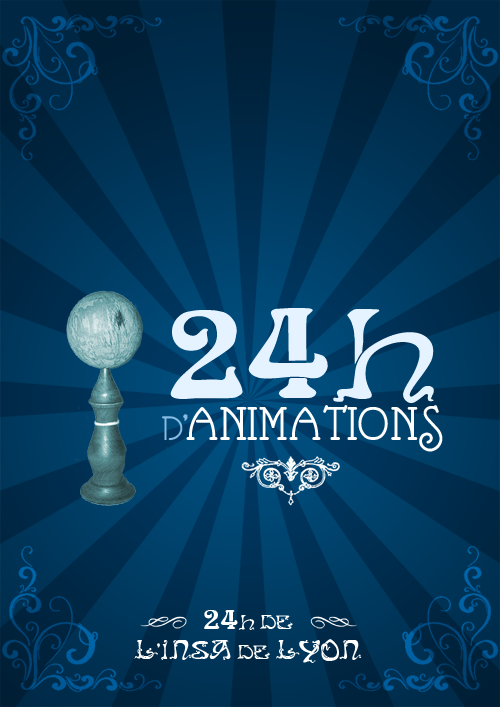
\includegraphics[width=0.3\textwidth]{img/old-preview-animations.png}}
                \fbox{
\includegraphics[width=0.3\textwidth]{img/old-preview-courses.png}}
                \fbox{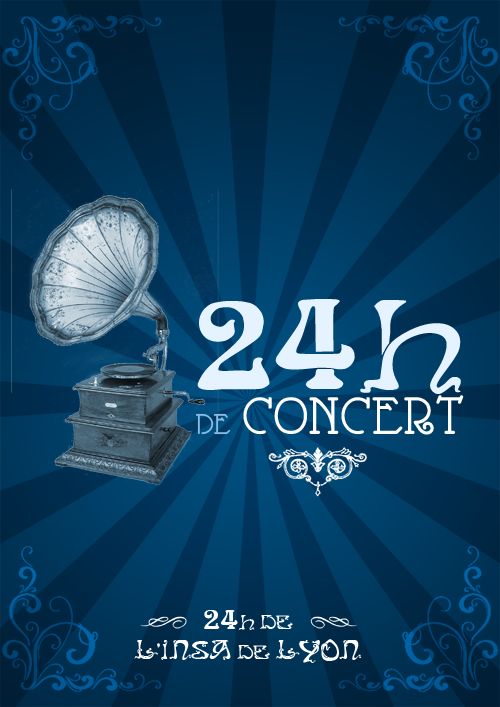
\includegraphics[width=0.3\textwidth]{img/old-preview-concert.png}}
            \end{center}
            Pendant la réalisation de l'affiche de la 36ème édition, j'ai réalisé, pour rigoler, une fausse affiche dans un style ancien, avec un grand-bi. En l'envoyant par mail à toutes l'équipes, j'ai été étonné de voir plusieurs réponses enthousiastes.
                J'ai donc retravaillé un peu le concept, et produit 3 affiches que j'ai présenté lors du choix du thème.            
            
            
            \begin{center}           
                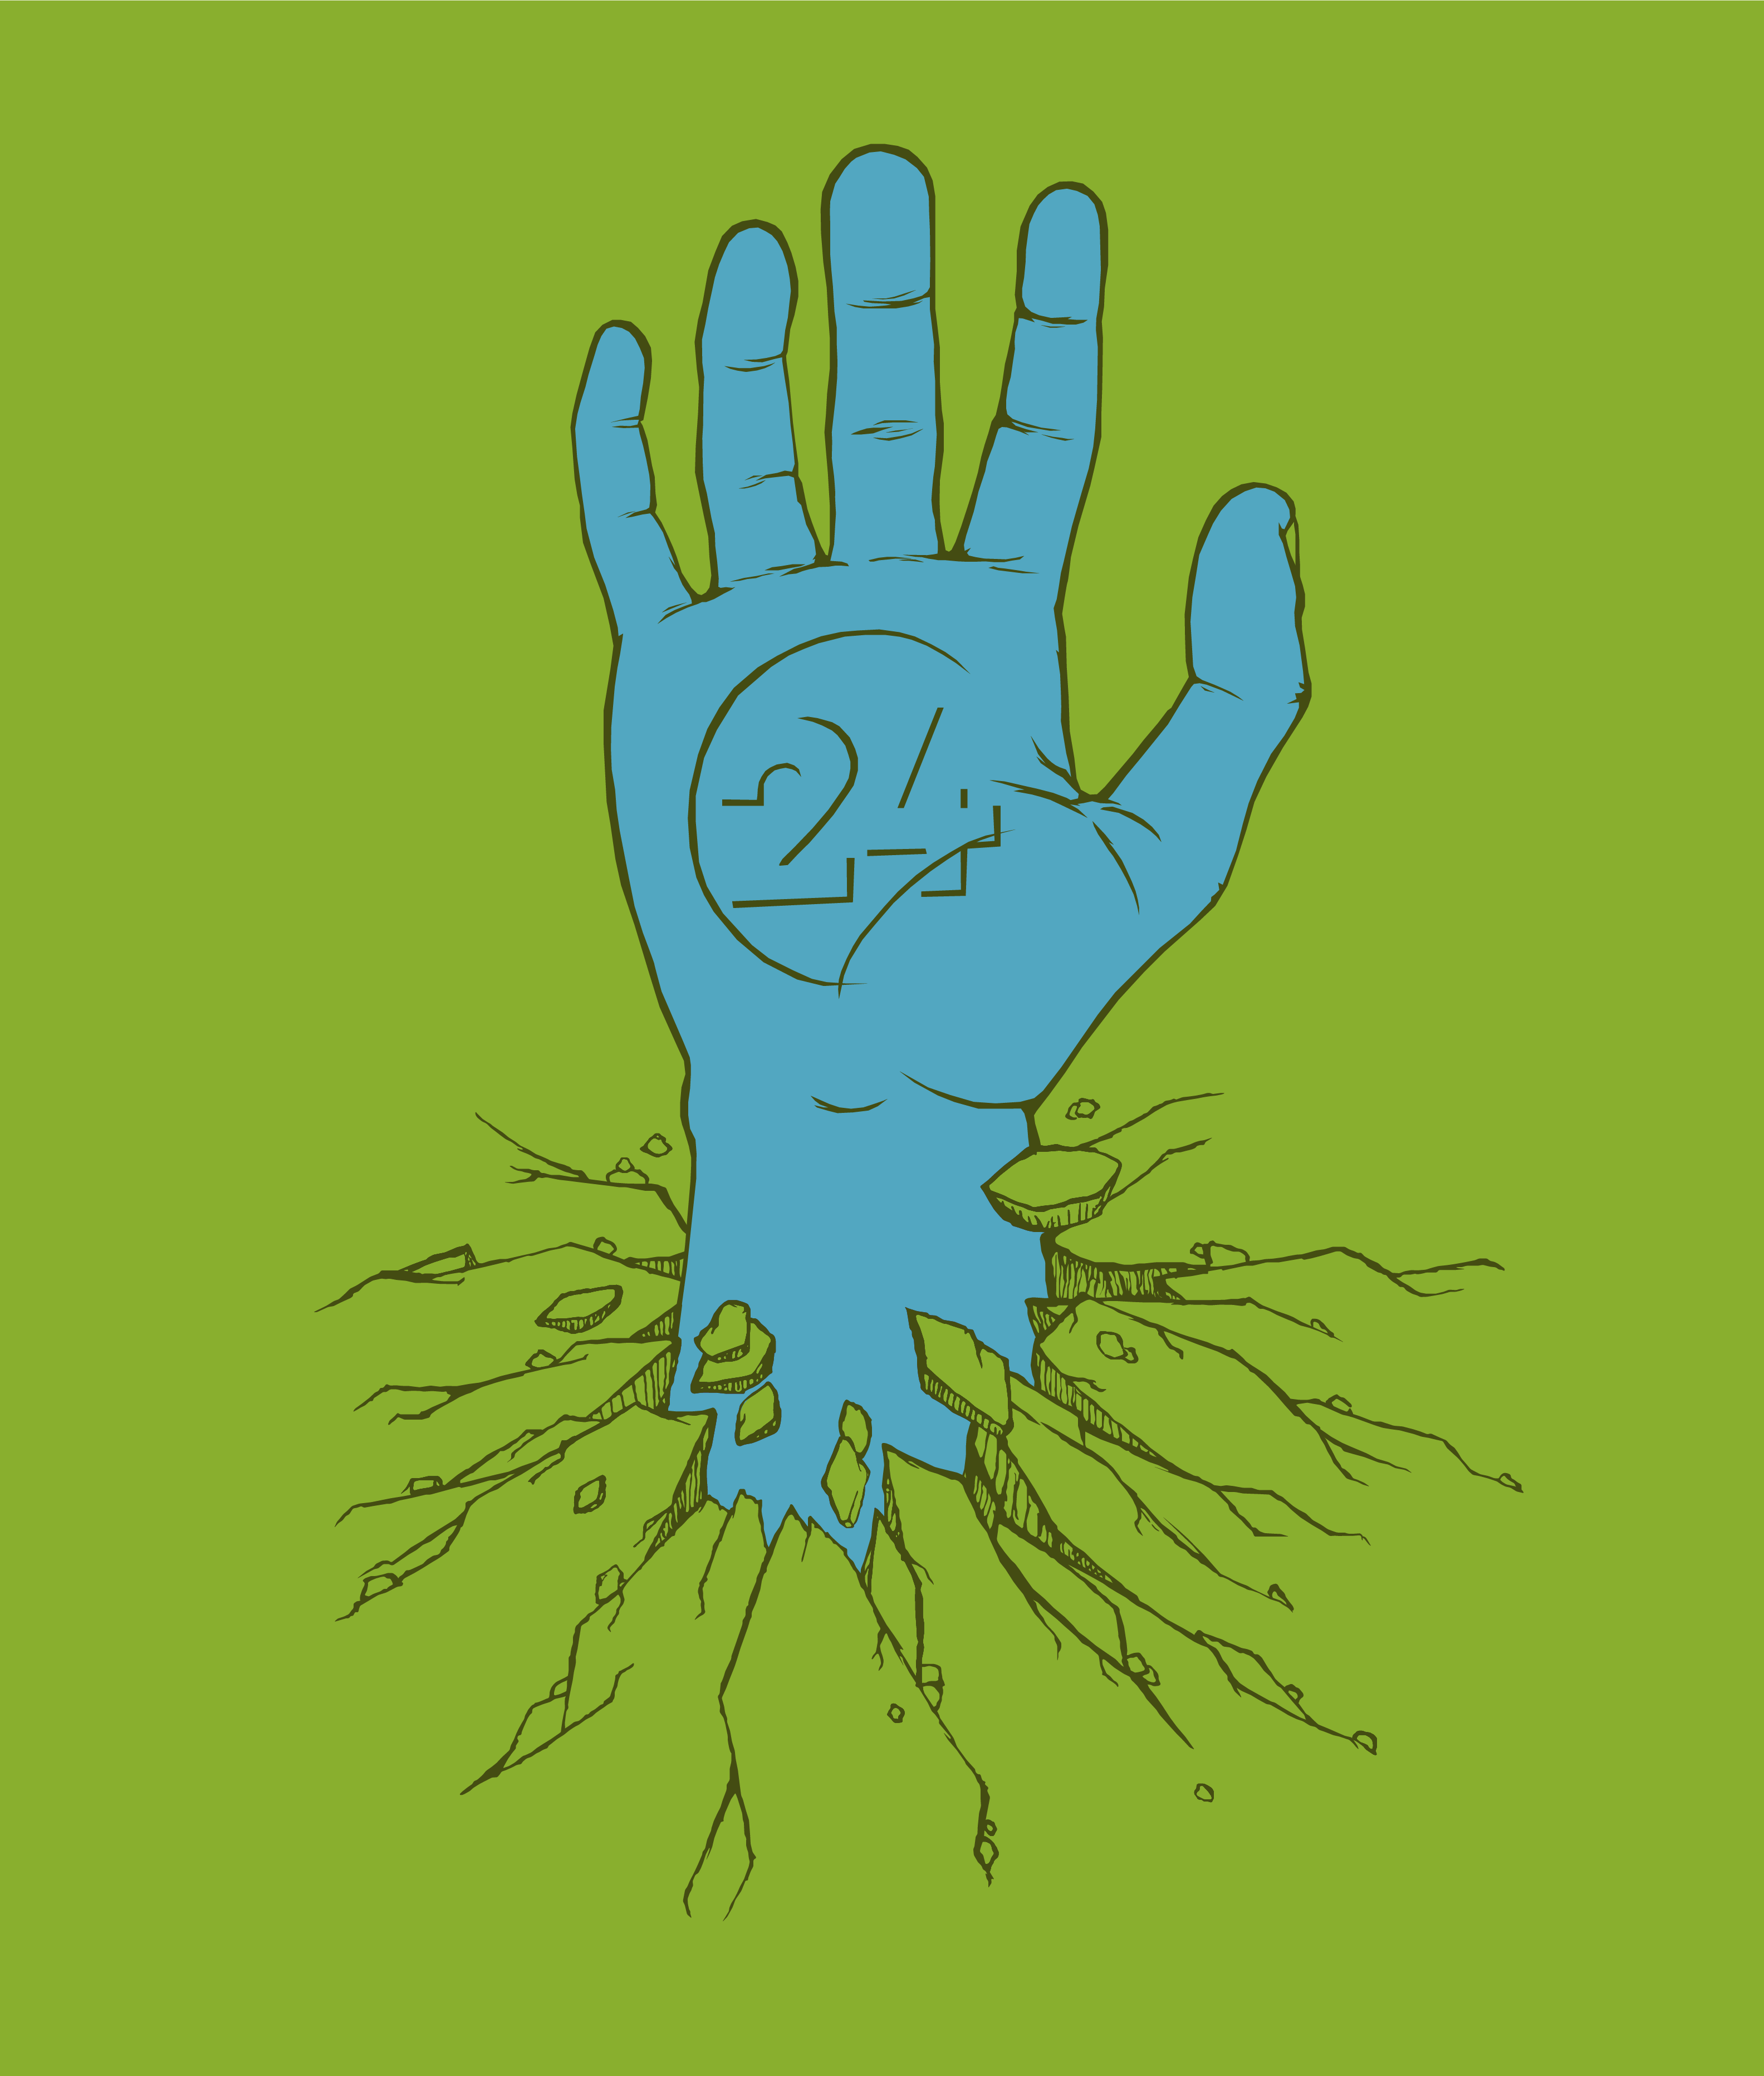
\includegraphics[width=\textwidth]{img/main.png}\\
                ~\\
                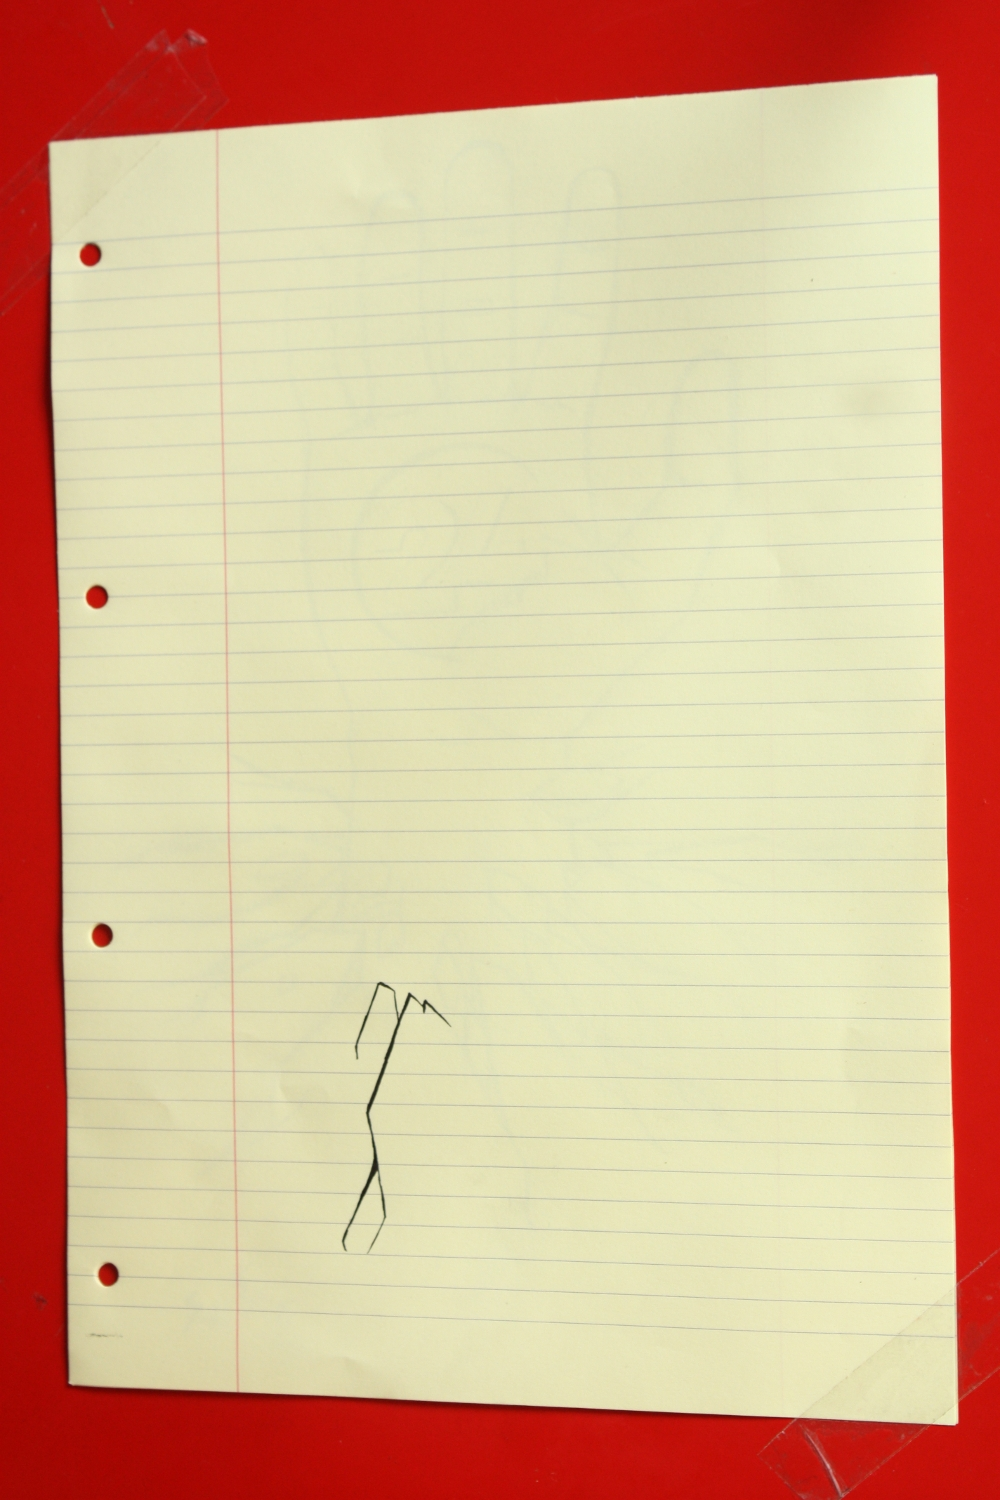
\includegraphics[width=0.24\textwidth]{img/IMG_5730.JPG}
                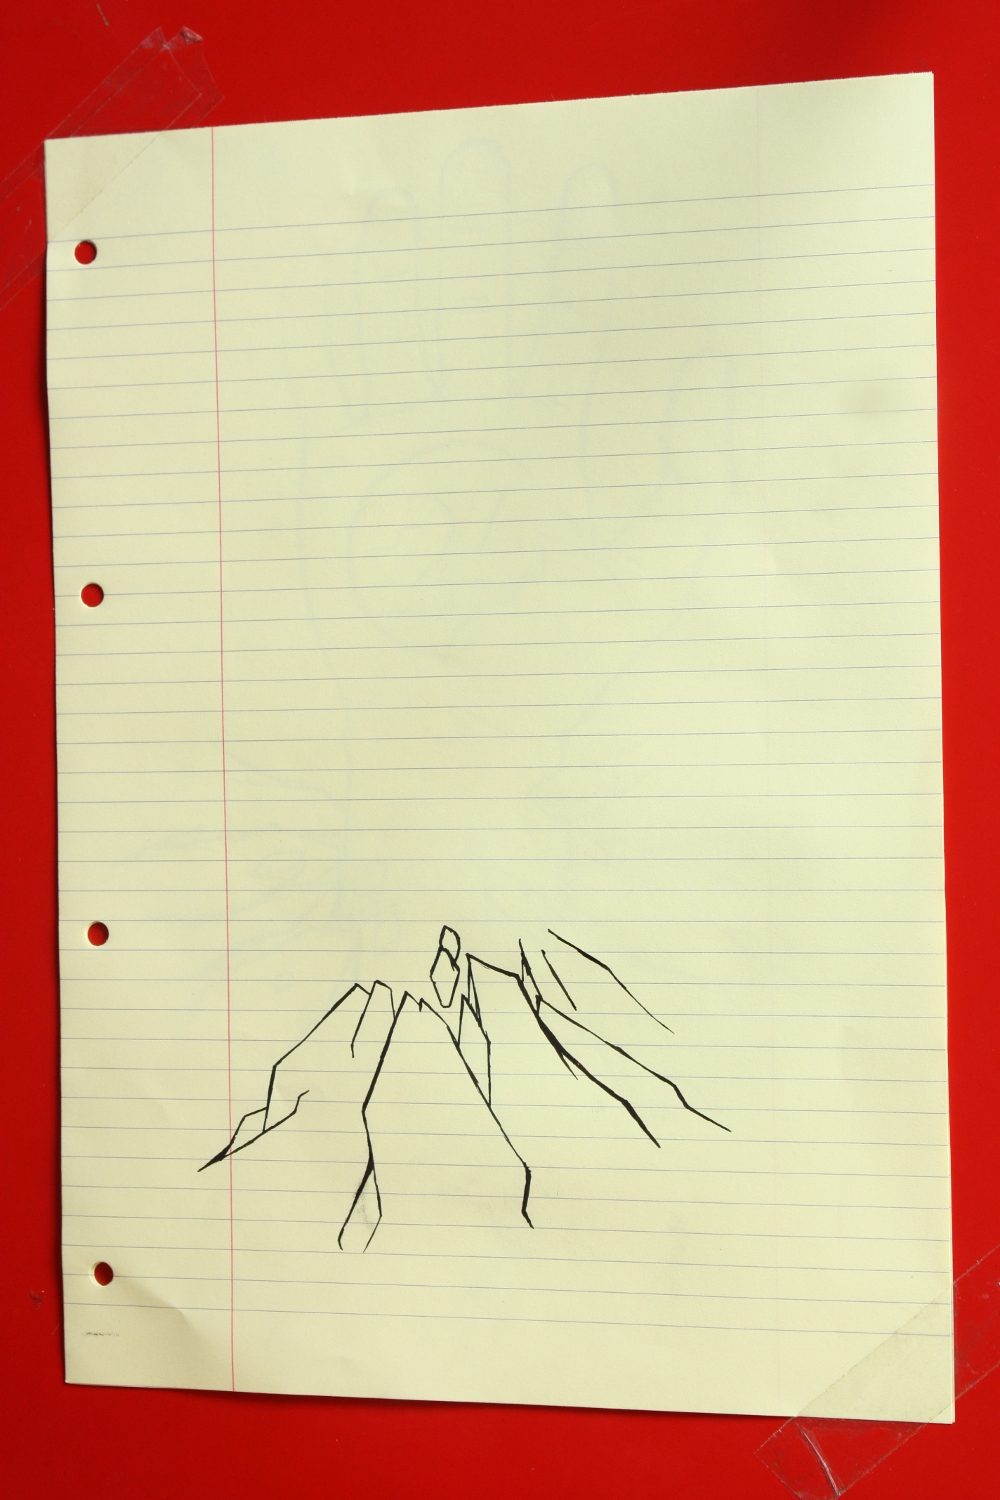
\includegraphics[width=0.24\textwidth]{img/IMG_5741.JPG}
                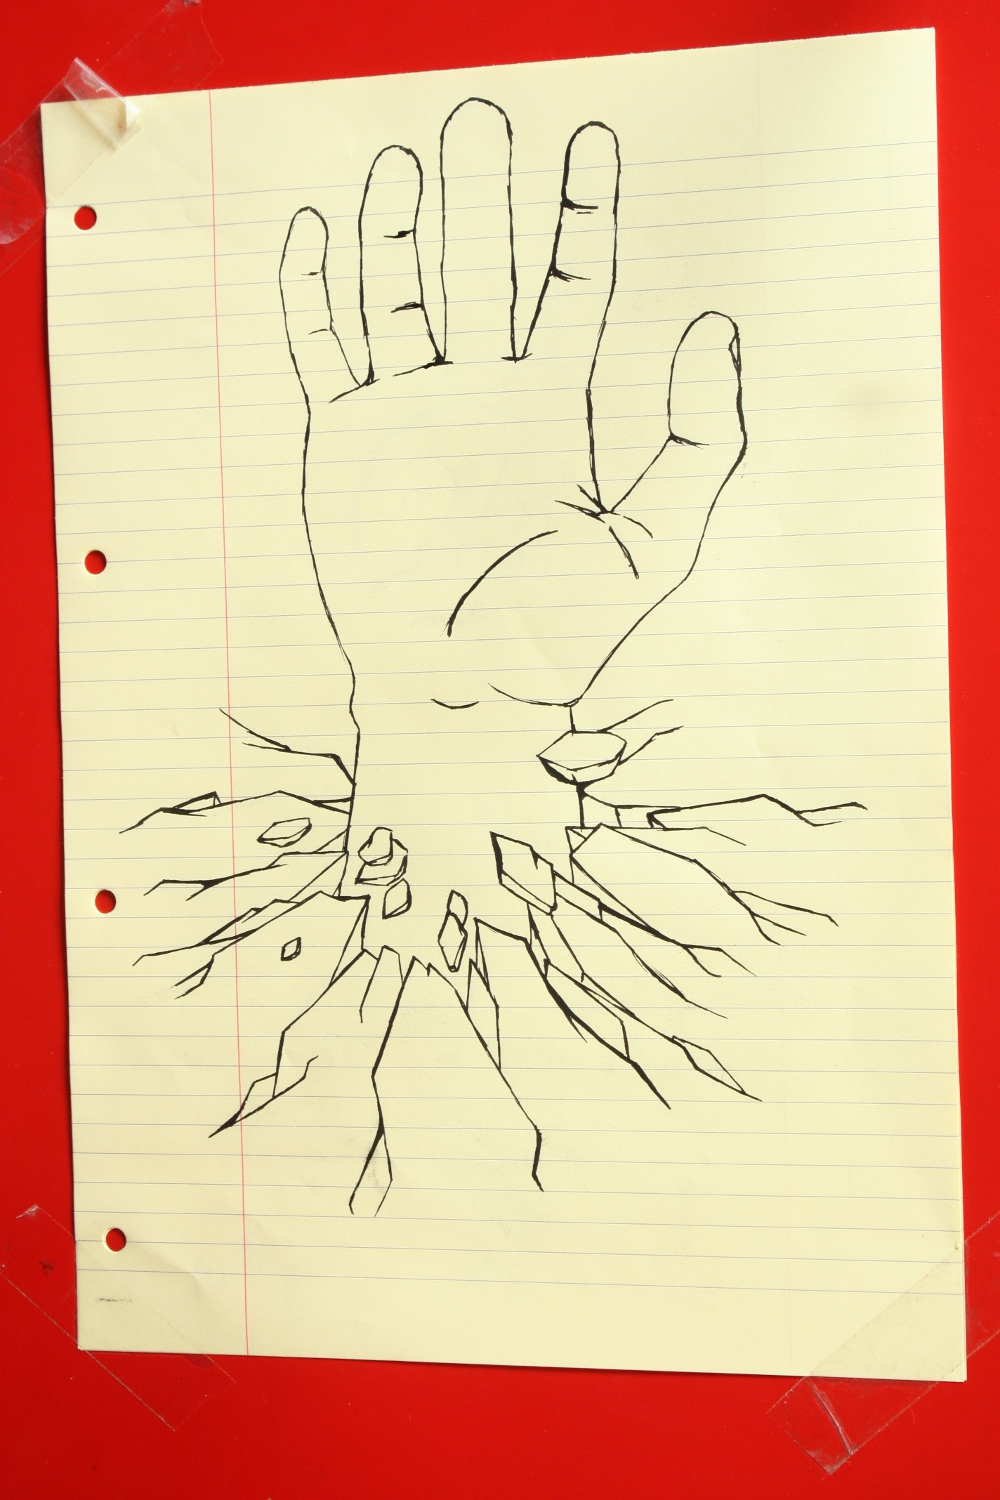
\includegraphics[width=0.24\textwidth]{img/IMG_5792.JPG}
                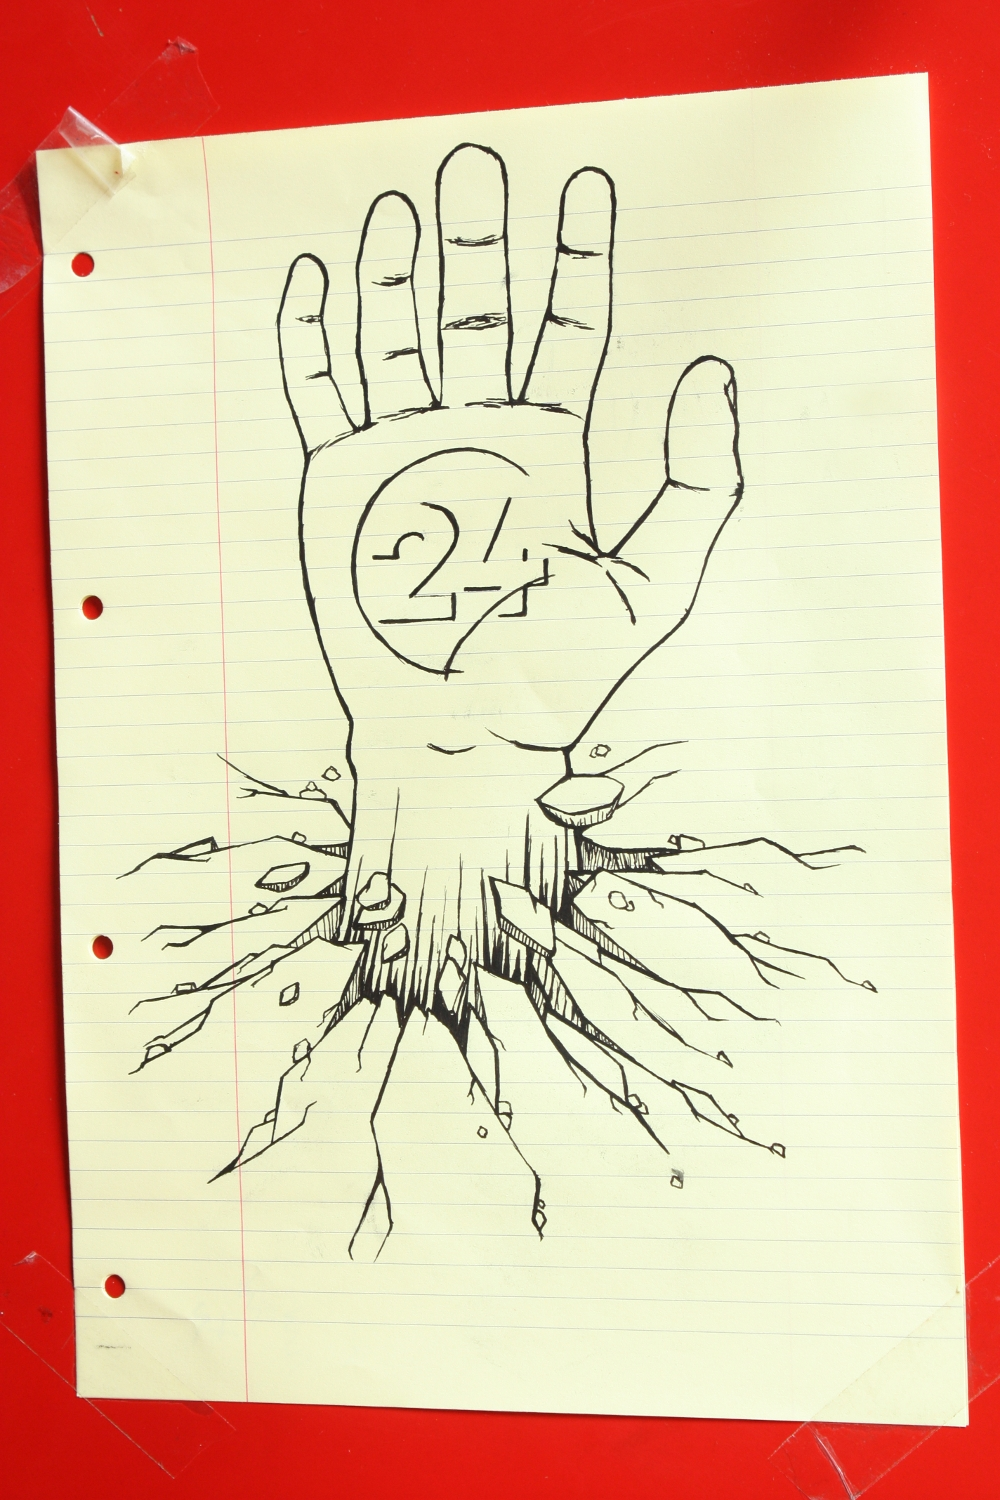
\includegraphics[width=0.24\textwidth]{img/IMG_5848.JPG}
            \end{center}
            Lors d'une réunion, nous discutions d'un visuel possible pour un des T-Shirt vente. Nous trouvions dynamique l'idée d'une main qui sortait de terre, avec des éclats volant un peu partout.
                J'ai réalisé un premier brouillon rapide pendant la réunion, je l'ai ensuite vectorisé et colorié pour obtenir ce résultat.
            
            \begin{center}                     
                
\includegraphics[width=\textwidth]{img/splash24.png}
            \end{center}
                Travail sur le logo de l'association, pour le thème \textit{tâches de peintures}.
                Le logo original, sans les tâches de peinture, est réutilisé depuis environ 6 ou 7 ans.
                Le fait d'y ajouter ces tâches de peinture n'empêche pas de reconnaître le logo original, et ajoute la cohérence nécessaire avec le thème.
                        
            \begin{center}
                
\includegraphics[width=\textwidth]{img/logo-TShirt-bichro.png}
            \end{center}
                Bien que ce visuel soit initialement prévu pour un T-Shirt, je l'ai dessiné comme si on l'utiliserais sur d'autres support moins exigeants.
                Basiquement, pour imprimer sur un T-Shirt, la seule contraintes à respecter est le nombre de couleurs, et parfois, les couleurs elle-mêmes.
                Nous avions un contrat avec notre imprimeur qui nous permettais de n'imprimer que 2 couleurs.
                Si on compte la couleur du T-Shirt en plus, on peut donc avoir 3 couleurs dans notre illustration.
                On voit bien sur ce visuel qu'il n'y a pas plus de 3 couleurs.
                Pourtant c'est le même visuel que le suivant, qui lui aurait été imprimé sur une affiche, donc sans toutes ces contraintes de couleurs.
                
            \begin{center}    
                \fbox{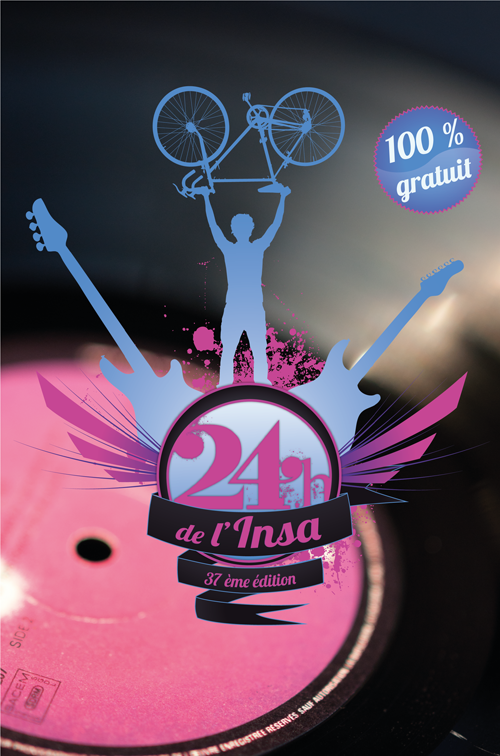
\includegraphics[width=\textwidth]{img/affiche-soiree.png}}
            \end{center}
            Ce visuel est le même que le précédent, cependant, j'ai changé les tons de couleurs, et fait apparaitres les dégradé. Contrairement à l'impression sur textile, l'impression sur papier est moins contraignante, il n'y as pas de limite de couleurs, et on peut utiliser des dégradés.
                La photo qui sert de fond à cette affiche, proviens de la série de photo prise pour l'affiche finale.
            
    \subsection{AEDI}
            
        \begin{center}
            %\fbox{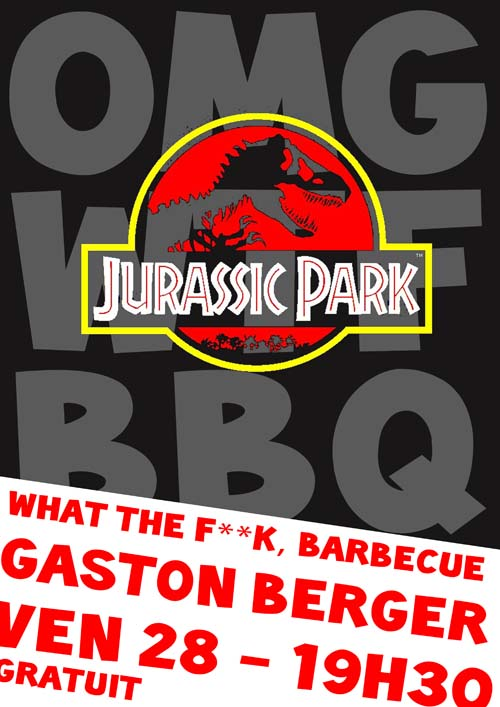
\includegraphics[width=0.3\textwidth]{img/WTFBBQjp.jpg}}
            \fbox{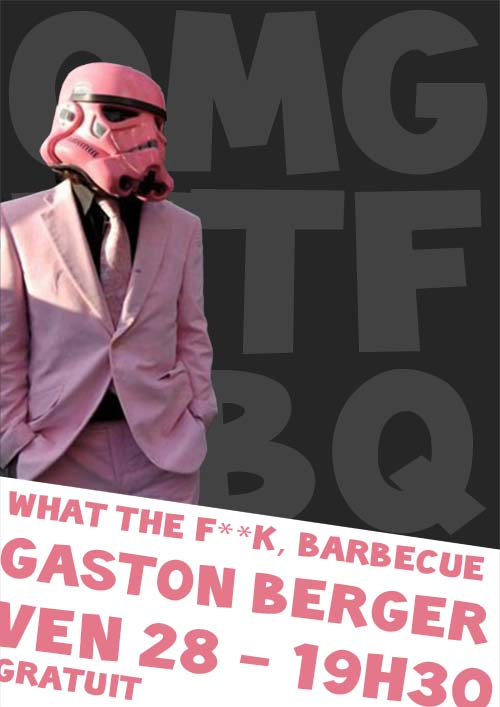
\includegraphics[width=0.3\textwidth]{img/WTFBBQstorm.jpg}}
            \fbox{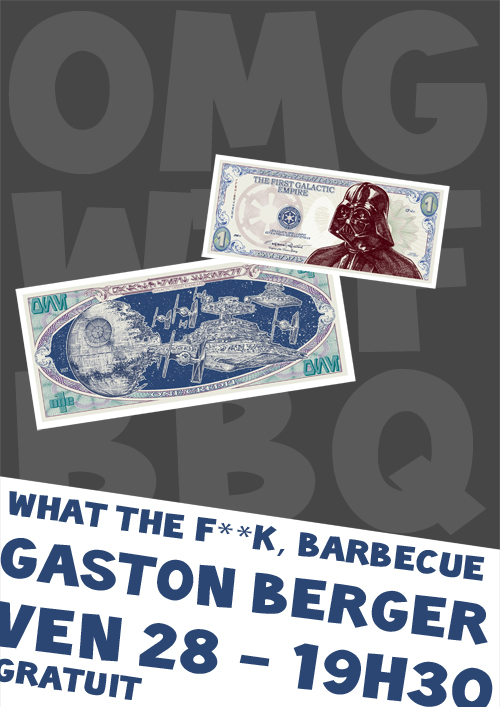
\includegraphics[width=0.3\textwidth]{img/WTFBBQsw.jpg}}
            %\fbox{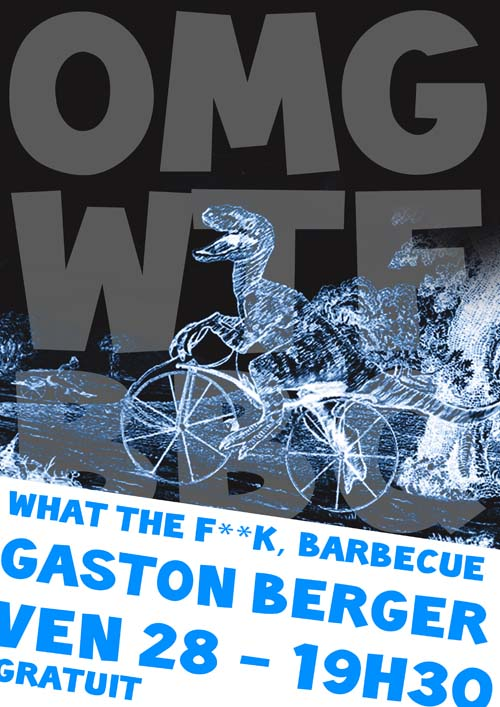
\includegraphics[width=0.3\textwidth]{img/WTFBBQvelo.jpg}}
            \fbox{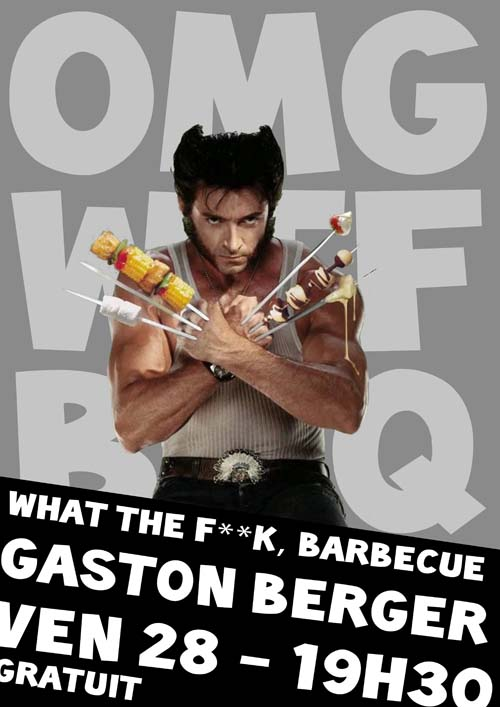
\includegraphics[width=0.3\textwidth]{img/WTFBBQwolv.jpg}}
            %\fbox{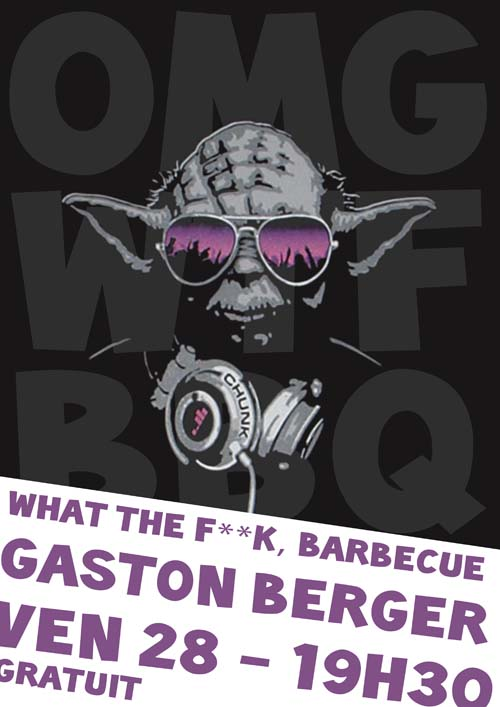
\includegraphics[width=0.3\textwidth]{img/WTFBBQyoda.jpg}}
        \end{center}
        Cette série d'affiche m'as été demandé par l'AEDI à l'occasion du barbecue du fin d'année.
            Le nom de l'évenement était : WTF OMG BBQ, et étant donné que c'est un barbecue organisé par le département informatique, chaque affiche est centré autour d'une référence \emph{Geek} détourné.
        
        \begin{center}
            \centering
            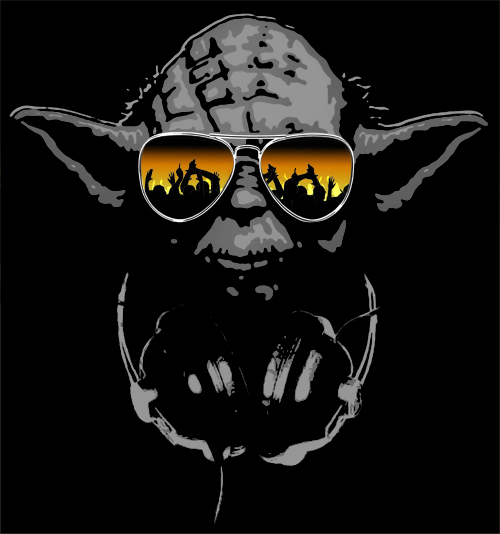
\includegraphics[width=0.9\textwidth]{img/yoda-or.jpg}\\
        \end{center}
            Initialement, cette image à été utilisé pour une des affiches du WTF OMG BBQ.
            Mais comme on était plusieurs (et moi particuliérement) à l'apprecier, on à décidé de la garder comme visuel de T-Shirt pour les \emph{bizuth} de la promotion 52.
            L'image de base, trouvé sur internet n'était pas d'assez bonne qualité, il m'as fallut la retoucher enormément, et remplacer la pluspart des éléments pour avoir une image ressemblante mais de bien meilleur qualité, prête pour l'impression.



